\ifx\mainfile\undefined
%  ========================================================================
%  Copyright (c) 2006-2011 The University of Washington
%
%  Licensed under the Apache License, Version 2.0 (the "License");
%  you may not use this file except in compliance with the License.
%  You may obtain a copy of the License at
%
%      http://www.apache.org/licenses/LICENSE-2.0
%
%  Unless required by applicable law or agreed to in writing, software
%  distributed under the License is distributed on an "AS IS" BASIS,
%  WITHOUT WARRANTIES OR CONDITIONS OF ANY KIND, either express or implied.
%  See the License for the specific language governing permissions and
%  limitations under the License.
%  ========================================================================
%
 
\documentclass [11pt, twoside] {uwthesis}

\usepackage{color}
\usepackage{url}
\usepackage{amsmath}
\usepackage{amsfonts}
\usepackage[bookmarks,
	hidelinks,
	plainpages=false,
	pdfpagelabels,
	pagebackref=true,
            ]{hyperref}
\renewcommand*{\backref}[1]{}% for backref < 1.33 necessary
\renewcommand*{\backrefalt}[4]{%
  \ifcase #1 %
    (No citations.)%
  \or
    (Cited on page #2.)%
  \else
    (Cited on pages #2.)%
  \fi
}

\newcommand{\biburl}[1]{{\tt<}\url{#1}{\tt>}}

\hypersetup{%
pdfauthor = {Daniel Chaim Halperin},
pdftitle = {Simplifying the Configuration of 802.11 Wireless Networks with Effective SNR},
pdfsubject = {Ph.D. Dissertation},
pdfkeywords = {},
pdfcreator = {University of Washington, Computer Science and Engineering},
pdfproducer = {},
bookmarksopen = {true},
pdfpagelayout = {TwoColumnRight},
}

\usepackage{footnotebackref}
%%%%%%%%%%%%%%%%%%%%%%%%%%%%%%%%%%%%%%%%%%%%%%%%%%%%%%
%%%        Formatting sections                     %%%
%%%%%%%%%%%%%%%%%%%%%%%%%%%%%%%%%%%%%%%%%%%%%%%%%%%%%%
\newcommand{\algref}[1]{Algorithm~\ref{#1}}
\newcommand{\chapref}[1]{Chapter~\ref{#1}}
\renewcommand{\eqref}[1]{Equation~\ref{#1}}
\newcommand{\figref}[1]{Figure~\ref{#1}}
\newcommand{\secref}[1]{\S\ref{#1}}
\newcommand{\tabref}[1]{Table~\ref{#1}}
\newcommand{\heading}[1]{\vspace{4pt}\noindent\textbf{#1}}
\newcommand{\topheading}[1]{\noindent\textbf{#1}}
\newcommand{\noheading}[0]{\vspace{4pt}\noindent}

%%%%%%%%%%%%%%%%%%%%%%%%%%%%%%%%%%%%%%%%%%%%%%%%%%%%%%
%%%        XXX and other warnings                  %%%
%%%%%%%%%%%%%%%%%%%%%%%%%%%%%%%%%%%%%%%%%%%%%%%%%%%%%%
\newcommand{\xxx}[1]{\textit{\color{red}XXX #1}}

%%%%%%%%%%%%%%%%%%%%%%%%%%%%%%%%%%%%%%%%%%%%%%%%%%%%%%
%%%        Units                                   %%%
%%%%%%%%%%%%%%%%%%%%%%%%%%%%%%%%%%%%%%%%%%%%%%%%%%%%%%
\usepackage{xspace}
\newcommand{\unitsep}{\texorpdfstring{\,}{ }}
\def\unit#1{% from: http://www.tex.ac.uk/cgi-bin/texfaq2html?label=csname "Defining a macro from an argument"
  \expandafter\def\csname #1\endcsname{\unitsep\text{#1}\xspace}%
}
\def\varunit#1#2{% from: http://www.tex.ac.uk/cgi-bin/texfaq2html?label=csname "Defining a macro from an argument"
  \expandafter\def\csname #1\endcsname{\unitsep\text{#2}\xspace}%
}
\unit{GHz}
\unit{MHz}
\unit{kHz}
\unit{Gbps}
\unit{Mbps}
\unit{KB}
\unit{dB}
\unit{dBi}
\unit{dBm}
\unit{W}
\unit{mW}
\varunit{uW}{$\mu$W}
\unit{ms}
\varunit{us}{$\mu$s}
\unit{h}
\unit{m}
\unit{s}
\unit{km}
\unit{cm}
\unit{mm}
\varunit{mmsq}{mm$^\text{2}$}
\varunit{insq}{in$^\text{2}$}
\newcommand{\degree}{\ensuremath{^\circ}\xspace}
\newcommand{\degrees}{\degree}
%%%%%%%%%%%%%%%%%%%%%%%%%%%%%%%%%%%%%%%%%%%%%%%%%%%%%%%%%%%%%%%%%%%%%%%%%%%%%%%%%%%%%%
% Euler for math | Palatino for rm | Helvetica for ss | Courier for tt
%
% From: http://www.tug.org/mactex/fonts/LaTeX_Preamble-Font_Choices.html
%%%%%%%%%%%%%%%%%%%%%%%%%%%%%%%%%%%%%%%%%%%%%%%%%%%%%%%%%%%%%%%%%%%%%%%%%%%%%%%%%%%%%%
\renewcommand{\rmdefault}{ppl} % rm
\usepackage[scaled]{helvet} % ss
\usepackage{courier} % tt
\usepackage{eulervm} % a better implementation of the euler package (not in gwTeX)
\normalfont
\usepackage[T1]{fontenc}
%%%%%%%%%%%%%%%%%%%%%%%%%%%%%%%%%%%%%%%%%%%%%%%%%%%%%%%%%%%%%%%%%%%%%%%%%%%%%%%%%%%%%%

%%%%%%%%%%%%%%%%%%%%%%%%%%%%%%%%%%%%%%%%%%%%%%%%%%%%%%
%%%        Figures                                 %%%
%%%%%%%%%%%%%%%%%%%%%%%%%%%%%%%%%%%%%%%%%%%%%%%%%%%%%%
\usepackage{graphicx}
% Caption package both lets you set the spacing between figure and caption
% and also makes the \figref{} point to the right place.
\usepackage[font=bf,aboveskip=6pt,belowskip=-4mm]{caption}
% Allow subfigures, make them bold
\usepackage[bf,BF,small]{subfigure}
% List of figures
\setcounter{lofdepth}{2}  % Print the chapter and sections to the lot

%%%%%%%%%%%%%%%%%%%%%%%%%%%%%%%%%%%%%%%%%%%%%%%%%%%%%%
%%%        Lists with reduced spacing              %%%
%%%%%%%%%%%%%%%%%%%%%%%%%%%%%%%%%%%%%%%%%%%%%%%%%%%%%%
\usepackage{enumitem}

%%%%%%%%%%%%%%%%%%%%%%%%%%%%%%%%%%%%%%%%%%%%%%%%%%%%%%
%%%        Fancy tables                            %%%
%%%%%%%%%%%%%%%%%%%%%%%%%%%%%%%%%%%%%%%%%%%%%%%%%%%%%%
\usepackage{tabulary}
\usepackage{booktabs}

%%%%%%%%%%%%%%%%%%%%%%%%%%%%%%%%%%%%%%%%%%%%%%%%%%%%%%
%%%        Formatting techniques/tools/etc.        %%%
%%%%%%%%%%%%%%%%%%%%%%%%%%%%%%%%%%%%%%%%%%%%%%%%%%%%%%
\newcommand{\term}[1]{\texttt{#1}}

\begin{document}
 
\textpages
\setcounter{chapter}{1} % Set to n-1!
\fi
%%%%%%%%%%%%%%%%%%%%%%%%%%%%%%%%%%

\cleardoublepage
\chapter{Background}
\label{chap:background}

\begin{table}
\centering
%\footnotesize
\begin{tabular}{cccc}
\toprule
MCS & Modulation & Coding Rate & Data Rate (Mbps) \\
\midrule
0 & BPSK & 1/2 & 6.5 \\
1 & QPSK & 1/2 & 13.0\\
2 & QPSK & 3/4 & 19.5\\
3 & 16-QAM & 1/2 & 26.0\\
4 & 16-QAM & 3/4 & 39.0\\
5 & 64-QAM & 2/3 & 52.0\\
6 & 64-QAM & 3/4 & 58.5\\
7 & 64-QAM & 5/6 & 65.0\\
\bottomrule
\end{tabular}
\caption[The 802.11n single-stream rates.]{\label{tab:siso_mcs} The single-stream 802.11n modulation and coding schemes. The first seven rates correspond to 802.11a/g rates (excluding 9\Mbps) with four added OFDM subcarriers; the highest data rate uses a new 5/6-rate code. The data rates are given for 20\MHz channels with 4\ms symbols.}
\end{table}

\section{Motivation: Inadequacy of RSSI}
\begin{figure}[t]
	\centering
\hfill%
		\subfigure[A wired 802.11n link with variable attenuation has a predictable relationship between SNR and packet reception rate (PRR) and clear separation between rates.]{
			\label{fig:snr_prr_attenuator}
			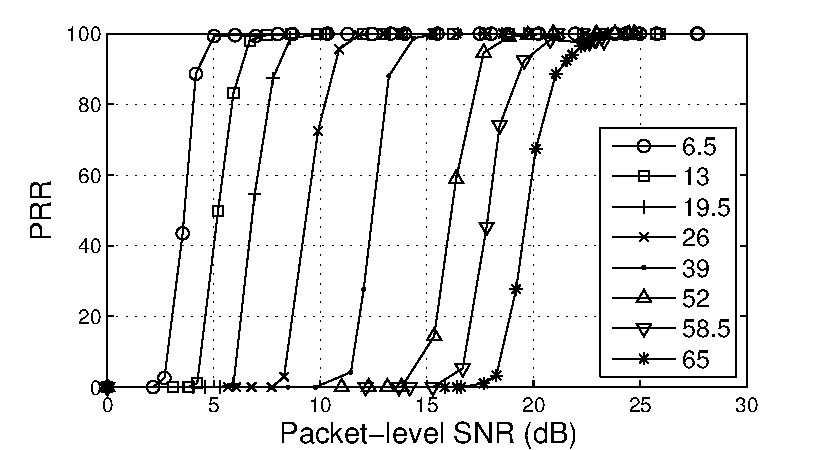
\includegraphics[width=0.4\textwidth,viewport=13 0 364 204,clip]{figures/esnr/embed_attenuator_snr_prr.pdf}
		}
\hfill%
      	\subfigure[Over real wireless channels in our testbeds, the transition region varies up to 10\dB. This loses the clear separation between rates (and so only three rates are shown for legibility).]{
			\label{fig:snr_prr_26_65}
			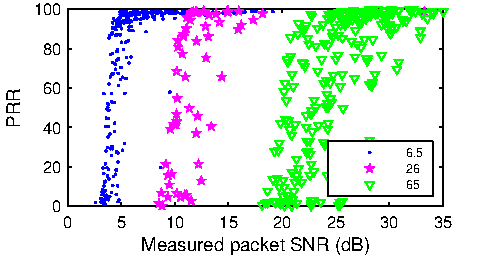
\includegraphics[width=0.4\textwidth,viewport=2 0 217 124,clip]{figures/esnr/embed_scatterplot_meas_snr_small.pdf}
		}
\hfill%
	\caption[Packet delivery over wired and real 802.11 channels]{\label{fig:rssi_predictions}Measured (single antenna) 802.11n packet delivery over wired and real channels.}%
\end{figure}
\topheading{Packet Delivery versus RSSI/SNR\@.}
Textbook analyses of modulation schemes give delivery probability for a single signal in terms of the signal-to-noise (SNR) ratio~\cite{Goldsmith}, %The SNR is defined as the ratio of the signal power to the thermal noise power, typically expressed on a logarithmic scale in decibels, i.e., SNR = $10\log_{10}(S/N)$. 
typically expressed on a log scale in decibels.
This model holds for narrowband channels with additive white Gaussian noise. It predicts a sharp transition region of 1--2\dB over which a link changes from extremely lossy to highly reliable. This makes the SNR a valuable indicator of performance.

We generated performance curves using SNR for the \term{iwl5300} over a simple wired link with a variable attenuator and for a single transmit and receive antenna. The result is shown for all single antenna 802.11n rates in \figref{fig:snr_prr_attenuator}. 
We observe a characteristic sharp transition region for packet reception rate (PRR) versus SNR\@. This is despite the relatively wide 20\MHz channel, 56 OFDM subcarriers, coding and other bit-level operations. This is the behavior we want from a link metric in order to predict packet delivery.

In contrast, packet delivery over real wireless channels does not exhibit the same picture. \figref{fig:snr_prr_26_65} shows the measured PRR versus SNR for three sample rates (6.5, 26, and 65\Mbps) over all wireless links in our testbeds, using the same 802.11n NICs. The SNR of the transition regions can exceed 10\dB, so that some links easily work for a given SNR and others do not. There is no longer clear separation between rates. This is consistent with other reported measurements that show RSSI does not predict packet delivery for real links~\cite{aguayo_roofnet, reis_sigcomm06, snr_infocom08, zhao_sensys03}.

%%%%%%%%%%%%%%%%%%%%%%%%%%%%%%%%%%
\ifx\mainfile\undefined
%
% ==========   Bibliography   ==========
%
%\nocite{*}   % include everything in the uwthesis.bib file
\bibliographystyle{plain}
\bibliography{dhalperi_thesis}

\end{document}
\fi
